%! TEX root = main.tex

\graphicspath{{00_Images/03_chapter/}}

\chapter{The Acoustic Domain}
\label{ch:acoustical_twoport}

The third domain in the transduction chain is the acoustical domain. Once the tools for mapping mechanical quantities to electrical ones are in place, extending the analogy to acoustics requires only identifying the correct power variables and deriving the constitutive relations for the three fundamental acoustic elements: mass, resistance, and compliance.

\section{Acoustic Variables and Fundamental Elements}
\label{sc:31}

The acoustical domain is characterized by two power variables. The acoustic pressure \(P\) (in pascal, \(\si{\pascal} = \si{\newton\per\meter\squared}\)) plays the role of the across-variable, analogous to voltage in the electrical domain or force in the mechanical domain. The volume velocity \(U\) (in \(\si{\cubic\meter\per\second}\)) plays the role of the through-variable, defined as:
\[
U = u \cdot S_D
\]
where \(u\) is the particle velocity and \(S_D\) is the cross-sectional area through which sound propagates. The instantaneous acoustic power flowing through a cross-section is:
\[
P_A = P \cdot U
\]
This is the direct acoustic counterpart of \(P_E = vi\) in the electrical domain and of \(P_M = Fu\) in the mechanical domain. The acoustic impedance of a one-port element is defined as:
\[
Z_A = \frac{P}{U}
\quad\left[\frac{\si{\pascal}}{\si{\cubic\meter\per\second}}
= \frac{\si{\newton\second}}{\si{\meter\tothe{5}}}\right]
\]
The specific acoustic impedance, which refers to particle velocity rather than volume velocity, is related to \(Z_A\) by \(Z_s = Z_A \cdot S\) and is measured in Rayls (\(\si{\pascal\second\per\meter}\)). For a plane wave in free air, the specific acoustic impedance equals the characteristic impedance of the medium, \(Z_0 = \rho_0 c \approx \SI{407}{\text{Rayl}}\).

\subsection{Acoustic Mass}
\label{ssc:311}

The acoustic mass \(M_A\) (in \(\si{\kilo\gram\per\meter\tothe{4}}\)) models the inertia of an air volume set in motion. It arises whenever a column of air is accelerated, for example inside a tube, a duct port, or the neck of a Helmholtz resonator. Starting from the mechanical equation \(F = M_M du/dt\) and substituting \(P = F/S\), \(U = uS\):
\[
M_A = \frac{M_M}{S^2}
\]
The acoustic constitutive relation is:
\[
P = M_A \frac{dU}{dt}
\qquad\Leftrightarrow\qquad
U(t) = \frac{1}{M_A}\int_0^t P(\tau) d\tau
\]
In sinusoidal operation the acoustic impedance of the mass is \(Z_{M_A} = j\omega M_A\), which increases linearly with frequency and dominates the acoustic response at high frequencies. The acoustic mass stores kinetic energy in the moving air slug but dissipates none.

\subsection{Acoustic Resistance}
\label{ssc:312}

The acoustic resistance \(R_A\) (in \(\si{\newton\second\per\meter\tothe{5}}\)) models the power dissipated by viscous friction as air flows through a constriction such as a porous material, a narrow tube, or the perforations of a diaphragm. Starting from the mechanical relation \(F = R_M u\) and substituting \(P = F/S\), \(U = uS\):
\[
R_A = \frac{R_M}{S^2}
\]
The acoustic constitutive relation is:
\[
P = R_A U
\qquad\Leftrightarrow\qquad
U = \frac{P}{R_A}
\]
Its acoustic impedance is purely real, \(Z_{R_A} = R_A\), independent of frequency, and mean acoustic power is dissipated at the rate \(\overline{P_A} = R_A U_{\mathrm{RMS}}^2\).

\paragraph{Practical example: perforated plate}
A rectangular block of height \(2b\), width \(w\), and depth \(t\), drilled with cylindrical holes of radius \(a\), presents both a resistive and a mass
contribution per hole. Under the impedance analogy these appear in series: \[
Z_A = R_A + j\omega M_A
\]
with analytical expressions:
\[
R_A = \frac{1}{\pi a^2}\sqrt{\frac{2\omega\mu}{\rho_0}}
\cdot\left[\frac{t}{a} + 2\!\left(1 - \frac{\pi a^2}{b^2}\right)\right],
\qquad
M_A = \frac{\rho_0}{\pi a^2}\left[t + 17a\!\left(1 - \frac{a}{b}\right)\right]
\]
where \(\mu\) is the dynamic viscosity of air. Such structures appear in loudspeaker cabinet design, microphone grilles, and acoustic absorption panels.

\subsection{Acoustic Compliance}
\label{ssc:313}

The acoustic compliance \(C_A\) (in \(\si{\meter\tothe{5}\per\newton}\)) models the elastic behavior of an enclosed volume of air. When a piston of area \(S\) compresses a cavity of volume \(V_0\), the restoring pressure is proportional to the fractional volume change, exactly as a mechanical spring restores a displaced mass. Starting from Hooke's law \(x = C_M F\), differentiating, and substituting \(U = uS\), \(P = F/S\):
\[
C_A = C_M S^2
\]
The acoustic constitutive relation is:
\[
U = C_A \frac{dP}{dt}
\qquad\Leftrightarrow\qquad
P(t) = \frac{1}{C_A}\int_0^t U(\tau) d\tau
\]
Its acoustic impedance is \(Z_{C_A} = 1/(j\omega C_A)\), which dominates the response at low frequencies. The acoustic compliance stores potential energy in the compressed air but dissipates none.

\begin{figure}[!htb]
    \centering
    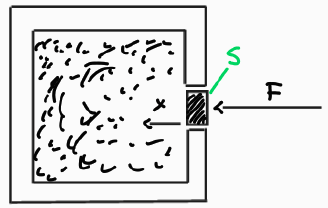
\includegraphics[width=0.5\linewidth]{acoustic_compliance_box.png}
    \caption{Acoustic compliance: a sealed box of volume \(V_0\) behind the
    diaphragm behaves as a spring. The equivalent acoustic compliance is
    \(C_A = V_0/(\rho_0 c^2)\) for an adiabatic process}
\end{figure}

For an adiabatic compression of an ideal gas in a rigid enclosure of volume \(V_0\), the acoustic compliance is:
\[
C_A = \frac{V_0}{\gamma P_0} = \frac{V_0}{\rho_0 c^2}
\]
where \(\gamma \approx 1.4\) is the ratio of specific heats, \(P_0 \approx \SI{101325}{\pascal}\) is the ambient pressure, and the equality \(\gamma P_0 = \rho_0 c^2\) holds for an adiabatic ideal gas. A larger box is more compliant, so its resonance with an acoustic mass occurs at a lower frequency, the physical basis for the dependence of a loudspeaker's bass response on enclosure volume.

\section{Acoustic Analogies}
\label{sc:32}

With the three acoustic elements defined, their mapping onto electrical circuit elements follows the same two analogies established in the mechanical domain. The acoustic power variables \((P, U)\) replace the mechanical pair \((F, u)\), and the acoustic impedance \(Z_A = P/U\) plays the same role as the mechanical impedance \(Z_M = F/u\).

\subsection{Impedance Analogy (Type I)}
\label{ssc:321}

The variable mapping is:
\[
P \;\leftrightarrow\; v, \qquad U \;\leftrightarrow\; i
\]
so that the acoustic impedance \(Z_A = P/U\) maps directly onto the electrical impedance \(Z_E = v/i\).

\paragraph{Acoustic Mass}
\[
P = M_A\frac{dU}{dt}
\;\xrightarrow{P\to v,\;U\to i}\;
v = M_A\frac{di}{dt} = L\frac{di}{dt}
\qquad\Longrightarrow\qquad
L_E = M_A
\]
The acoustic mass corresponds to an inductor.

\paragraph{Acoustic Resistance}
\[
P = R_A U
\;\xrightarrow{P\to v,\;U\to i}\;
v = R_A i
\qquad\Longrightarrow\qquad
R_E = R_A
\]
The acoustic resistance corresponds to a resistor.

\paragraph{Acoustic Compliance}
\[
U = C_A\frac{dP}{dt}
\;\xrightarrow{U\to i,\;P\to v}\;
i = C_A\frac{dv}{dt} = C\frac{dv}{dt}
\qquad\Longrightarrow\qquad
C_E = C_A
\]
The acoustic compliance corresponds to a capacitor.

\paragraph{Summary and topological rule}
\[
M_A \;\leftrightarrow\; L_E,
\qquad C_A \;\leftrightarrow\; C_E,
\qquad R_A \;\leftrightarrow\; R_E
\]
Since volume velocity maps to current, acoustic elements sharing the same volume velocity are connected in series in the equivalent circuit.

\subsection{Admittance Analogy (Type II)}
\label{ssc:322}

The variable mapping is:
\[
P \;\leftrightarrow\; i, \qquad U \;\leftrightarrow\; v
\]
so that the acoustic admittance \(Y_A = U/P\) maps directly onto the electrical admittance \(Y_E = i/v\).

\paragraph{Acoustic Mass}
\[
P = M_A\frac{dU}{dt}
\;\xrightarrow{P\to i,\;U\to v}\;
i = M_A\frac{dv}{dt} = C\frac{dv}{dt}
\qquad\Longrightarrow\qquad
C_E = M_A
\]
The acoustic mass corresponds to a capacitor.

\paragraph{Acoustic Resistance}
\[
P = R_A U
\;\xrightarrow{P\to i,\;U\to v}\;
i = R_A v
\qquad\Longrightarrow\qquad
G_E = R_A, \quad R_E = \frac{1}{R_A}
\]
The acoustic resistance corresponds to a conductance \(G_E = R_A\), represented in circuit diagrams as a resistor of value \(R_E = 1/R_A\).

\paragraph{Acoustic Compliance}
\[
U = C_A\frac{dP}{dt}
\;\xrightarrow{U\to v,\;P\to i}\;
v = C_A\frac{di}{dt} = L\frac{di}{dt}
\qquad\Longrightarrow\qquad
L_E = C_A
\]
The acoustic compliance corresponds to an inductor.

\paragraph{Summary and topological rule}
\[
M_A \;\leftrightarrow\; C_E,
\qquad C_A \;\leftrightarrow\; L_E,
\qquad R_A \;\leftrightarrow\; G_E
\]
Since volume velocity maps to voltage, acoustic elements sharing the same volume velocity are connected in parallel in the equivalent circuit.

\subsection{Summary of the Two Analogies}
\label{ssc:323}

Both analogies are mathematically equivalent and produce identical predictions for all physical observables once the correct network topology is adopted. The choice is governed by the natural topology of the system under analysis.

\begin{table}[!htb]
\centering
\renewcommand{\arraystretch}{1.3}
\begin{tabular}{|c|c|c|}
\hline
\textbf{Acoustic element} & \textbf{Impedance analogy} & \textbf{Admittance analogy} \\
                          & T\textbf{ype I}            & \textbf{Type II} \\
\hline
Pressure \(P\)       & Voltage \(v\) & Current \(i\) \\
Volume velocity \(U\) & Current \(i\) & Voltage \(v\) \\
\hline
Mass \(M_A\)        & Inductor \(L_E = M_A\)          & Capacitor \(C_E = M_A\) \\
Compliance \(C_A\)  & Capacitor \(C_E = C_A\)          & Inductor \(L_E = C_A\)  \\
Resistance \(R_A\)  & Resistor \(R_E = R_A\)           & Conductance \(G_E = R_A\) \\
\hline
Common-\(U\) elements & Series circuit & Parallel circuit \\
\hline
\end{tabular}
\caption{Variable mappings and element correspondences for the impedance analogy
(Type I) and the admittance analogy (Type II) in the acoustic domain. Both
analogies are physically equivalent; the choice is one of topological
convenience}
\label{tab:acousticAnalogies}
\end{table}

\paragraph{Acoustic impedance and power} Regardless of which analogy is chosen,
the acoustic impedance of a one-port element is:
\[
Z_A = \frac{P}{U} = R_A + jX_A
\]
where \(R_A\) is the resistive (power-dissipating) part and \(X_A = \omega M_A - 1/(\omega C_A)\) is the reactive (energy-storing) part. The mean acoustic power delivered to the element is:
\[
\overline{P_A} = R_A U_{\mathrm{RMS}}^2
\]
confirming that only the resistive part of the acoustic impedance contributes to net energy dissipation, in complete analogy with the electrical case \(\overline{P_E} = \mathcal{R}\{Z_E\} I_{\mathrm{RMS}}^2\) and the mechanical case \(\overline{P_M} = R_M u_{\mathrm{RMS}}^2\).
